\documentclass[twoside]{book}

% Packages required by doxygen
\usepackage{fixltx2e}
\usepackage{calc}
\usepackage{doxygen}
\usepackage[export]{adjustbox} % also loads graphicx
\usepackage{graphicx}
\usepackage[utf8]{inputenc}
\usepackage{makeidx}
\usepackage{multicol}
\usepackage{multirow}
\PassOptionsToPackage{warn}{textcomp}
\usepackage{textcomp}
\usepackage[nointegrals]{wasysym}
\usepackage[table]{xcolor}

% Font selection
\usepackage[T1]{fontenc}
\usepackage[scaled=.90]{helvet}
\usepackage{courier}
\usepackage{amssymb}
\usepackage{sectsty}
\renewcommand{\familydefault}{\sfdefault}
\allsectionsfont{%
  \fontseries{bc}\selectfont%
  \color{darkgray}%
}
\renewcommand{\DoxyLabelFont}{%
  \fontseries{bc}\selectfont%
  \color{darkgray}%
}
\newcommand{\+}{\discretionary{\mbox{\scriptsize$\hookleftarrow$}}{}{}}

% Page & text layout
\usepackage{geometry}
\geometry{%
  a4paper,%
  top=2.5cm,%
  bottom=2.5cm,%
  left=2.5cm,%
  right=2.5cm%
}
\tolerance=750
\hfuzz=15pt
\hbadness=750
\setlength{\emergencystretch}{15pt}
\setlength{\parindent}{0cm}
\setlength{\parskip}{0.2cm}
\makeatletter
\renewcommand{\paragraph}{%
  \@startsection{paragraph}{4}{0ex}{-1.0ex}{1.0ex}{%
    \normalfont\normalsize\bfseries\SS@parafont%
  }%
}
\renewcommand{\subparagraph}{%
  \@startsection{subparagraph}{5}{0ex}{-1.0ex}{1.0ex}{%
    \normalfont\normalsize\bfseries\SS@subparafont%
  }%
}
\makeatother

% Headers & footers
\usepackage{fancyhdr}
\pagestyle{fancyplain}
\fancyhead[LE]{\fancyplain{}{\bfseries\thepage}}
\fancyhead[CE]{\fancyplain{}{}}
\fancyhead[RE]{\fancyplain{}{\bfseries\leftmark}}
\fancyhead[LO]{\fancyplain{}{\bfseries\rightmark}}
\fancyhead[CO]{\fancyplain{}{}}
\fancyhead[RO]{\fancyplain{}{\bfseries\thepage}}
\fancyfoot[LE]{\fancyplain{}{}}
\fancyfoot[CE]{\fancyplain{}{}}
\fancyfoot[RE]{\fancyplain{}{\bfseries\scriptsize Generated on Fri May 6 2016 18\+:37\+:30 for Li\+D\+A\+R Modeling Engine by Doxygen }}
\fancyfoot[LO]{\fancyplain{}{\bfseries\scriptsize Generated on Fri May 6 2016 18\+:37\+:30 for Li\+D\+A\+R Modeling Engine by Doxygen }}
\fancyfoot[CO]{\fancyplain{}{}}
\fancyfoot[RO]{\fancyplain{}{}}
\renewcommand{\footrulewidth}{0.4pt}
\renewcommand{\chaptermark}[1]{%
  \markboth{#1}{}%
}
\renewcommand{\sectionmark}[1]{%
  \markright{\thesection\ #1}%
}

% Indices & bibliography
\usepackage{natbib}
\usepackage[titles]{tocloft}
\setcounter{tocdepth}{3}
\setcounter{secnumdepth}{5}
\makeindex

% Hyperlinks (required, but should be loaded last)
\usepackage{ifpdf}
\ifpdf
  \usepackage[pdftex,pagebackref=true]{hyperref}
\else
  \usepackage[ps2pdf,pagebackref=true]{hyperref}
\fi
\hypersetup{%
  colorlinks=true,%
  linkcolor=blue,%
  citecolor=blue,%
  unicode%
}

% Custom commands
\newcommand{\clearemptydoublepage}{%
  \newpage{\pagestyle{empty}\cleardoublepage}%
}


%===== C O N T E N T S =====

\begin{document}

% Titlepage & ToC
\hypersetup{pageanchor=false,
             bookmarks=true,
             bookmarksnumbered=true,
             pdfencoding=unicode
            }
\pagenumbering{roman}
\begin{titlepage}
\vspace*{7cm}
\begin{center}%
{\Large Li\+D\+A\+R Modeling Engine \\[1ex]\large 0.\+0.\+1 }\\
\vspace*{1cm}
{\large Generated by Doxygen 1.8.9.1}\\
\vspace*{0.5cm}
{\small Fri May 6 2016 18:37:30}\\
\end{center}
\end{titlepage}
\clearemptydoublepage
\tableofcontents
\clearemptydoublepage
\pagenumbering{arabic}
\hypersetup{pageanchor=true}

%--- Begin generated contents ---
\chapter{Li\+D\+A\+R Modeling Engine}
\label{d5/d26/md__home_ncasler_apps_DSME_README}
\hypertarget{d5/d26/md__home_ncasler_apps_DSME_README}{}
This library is intended to ease the manipulation and processing of large lidar collections through a set of parallelized methods which interface between the datasets and a H\+D\+F5 data store.

\subsection*{Dependencies }

Z\+L\+I\+B\+: compression library M\+P\+I\+: Message passing library H\+D\+F5\+: Hierarchical Data Format(compiled with parallel support) Lib\+L\+A\+S\+: L\+A\+S data manipulation library G\+E\+O\+S\+: Geometric Topology library Proj.\+4\+: Projection transformation library G\+D\+A\+L\+: Geograpic Data Abstraction Library (compiled with external libgeotiff) Lib\+Geo\+Tiff\+: Geographic T\+I\+F\+F driver

\subsection*{Architecture }

{\itshape L\+M\+E Datastore}\+: Central data repository for lidar derivatives and metadata, keeps track of datasets and user access privileges. Needed to efficiently distribute processing to system.

{\itshape Li\+D\+A\+R Region}\+: A class which represents a geographic domain with Li\+D\+A\+R coverage. These regions will have administrators and user access privileges. The region will be initialized with a directory that contains Li\+D\+A\+R datasets.

{\itshape Dataset}\+: A Li\+D\+A\+R dataset (typically L\+A\+S format) which is registered for processing.

{\itshape Derivative}\+: A gridded dataset created by interpolating a subset of Li\+D\+A\+R points from an area. This derivative will be owned by the user that requested the data.

\subsection*{Workflow }


\begin{DoxyEnumerate}
\item Initialize Data\+Store
\item Register a Li\+D\+A\+R region
\item Request subset
\item Download result(or view a T\+M\+S online) 
\end{DoxyEnumerate}
\chapter{B\+U\+G\+S}
\label{d4/d48/md__home_ncasler_apps_DSME_TODO}
\hypertarget{d4/d48/md__home_ncasler_apps_DSME_TODO}{}
\subsubsection*{Read\+Header\+Block}

Should properly balance headers between processes -\/$>$ Fast enough for now \subsubsection*{Implement proper Hilbert index}

current implementation is functions, but need to find method to query indexes

\subsubsection*{Update reading process to insert reference to the point\textquotesingle{}s source file}

\subsection*{T\+O\+D\+O}

\subsubsection*{Merge\+Sort}

Implement mergesort into the reading phase

\subsubsection*{Rtree based on indexes -\/$>$ 50\% Complete}

\subsubsection*{Read point files based on area and clip point -\/$>$ D\+O\+N\+E}
\chapter{Data Structure Index}
\section{Data Structures}
Here are the data structures with brief descriptions\+:\begin{DoxyCompactList}
\item\contentsline{section}{\hyperlink{structbound__dbl__t}{bound\+\_\+dbl\+\_\+t} }{\pageref{d3/dcf/structbound__dbl__t}}{}
\item\contentsline{section}{\hyperlink{structbound__t}{bound\+\_\+t} }{\pageref{da/d1a/structbound__t}}{}
\item\contentsline{section}{\hyperlink{structcolor__t}{color\+\_\+t} }{\pageref{d8/dcc/structcolor__t}}{}
\item\contentsline{section}{\hyperlink{structcoord__dbl__t}{coord\+\_\+dbl\+\_\+t} }{\pageref{db/de5/structcoord__dbl__t}}{}
\item\contentsline{section}{\hyperlink{structcoord__t}{coord\+\_\+t} }{\pageref{d9/dec/structcoord__t}}{}
\item\contentsline{section}{\hyperlink{structfilter__t}{filter\+\_\+t} }{\pageref{d8/dff/structfilter__t}}{}
\item\contentsline{section}{\hyperlink{structHcode}{Hcode} }{\pageref{dd/d41/structHcode}}{}
\item\contentsline{section}{\hyperlink{structheader__t}{header\+\_\+t} }{\pageref{de/d7e/structheader__t}}{}
\item\contentsline{section}{\hyperlink{structJobstat}{Jobstat} }{\pageref{d7/dc3/structJobstat}}{}
\item\contentsline{section}{\hyperlink{structopdata}{opdata} }{\pageref{d5/da3/structopdata}}{}
\item\contentsline{section}{\hyperlink{structPoint}{Point} }{\pageref{d8/d43/structPoint}}{}
\item\contentsline{section}{\hyperlink{structproj__t}{proj\+\_\+t} }{\pageref{d7/db2/structproj__t}}{}
\item\contentsline{section}{\hyperlink{structreturn__t}{return\+\_\+t} }{\pageref{d1/da3/structreturn__t}}{}
\item\contentsline{section}{\hyperlink{structtask__t}{task\+\_\+t} }{\pageref{d6/daa/structtask__t}}{}
\end{DoxyCompactList}

\chapter{File Index}
\section{File List}
Here is a list of all documented files with brief descriptions\+:\begin{DoxyCompactList}
\item\contentsline{section}{/home/ncasler/apps/\+D\+S\+M\+E/include/{\bfseries bound.\+h} }{\pageref{df/dfb/bound_8h}}{}
\item\contentsline{section}{/home/ncasler/apps/\+D\+S\+M\+E/include/{\bfseries common.\+h} }{\pageref{dc/d54/common_8h}}{}
\item\contentsline{section}{/home/ncasler/apps/\+D\+S\+M\+E/include/{\bfseries file\+\_\+util.\+h} }{\pageref{d0/dae/file__util_8h}}{}
\item\contentsline{section}{/home/ncasler/apps/\+D\+S\+M\+E/include/{\bfseries filter.\+h} }{\pageref{dd/de7/filter_8h}}{}
\item\contentsline{section}{/home/ncasler/apps/\+D\+S\+M\+E/include/{\bfseries header.\+h} }{\pageref{df/dcb/header_8h}}{}
\item\contentsline{section}{/home/ncasler/apps/\+D\+S\+M\+E/include/{\bfseries hilbert.\+h} }{\pageref{dc/dba/hilbert_8h}}{}
\item\contentsline{section}{/home/ncasler/apps/\+D\+S\+M\+E/include/{\bfseries point.\+h} }{\pageref{d2/d91/point_8h}}{}
\item\contentsline{section}{/home/ncasler/apps/\+D\+S\+M\+E/include/{\bfseries reader.\+h} }{\pageref{d6/dda/reader_8h}}{}
\item\contentsline{section}{/home/ncasler/apps/\+D\+S\+M\+E/include/{\bfseries util.\+h} }{\pageref{d8/d3c/util_8h}}{}
\item\contentsline{section}{/home/ncasler/apps/\+D\+S\+M\+E/src/\hyperlink{bound_8c}{bound.\+c} \\*File containing methods for the bound object }{\pageref{dc/d00/bound_8c}}{}
\item\contentsline{section}{/home/ncasler/apps/\+D\+S\+M\+E/src/\hyperlink{common_8c}{common.\+c} \\*File containing common utility functions }{\pageref{d8/d19/common_8c}}{}
\item\contentsline{section}{/home/ncasler/apps/\+D\+S\+M\+E/src/\hyperlink{filter_8c}{filter.\+c} \\*File containing point filtration methods }{\pageref{d2/d4d/filter_8c}}{}
\item\contentsline{section}{/home/ncasler/apps/\+D\+S\+M\+E/src/\hyperlink{header_8c}{header.\+c} \\*File containing methods for reading header data }{\pageref{df/db9/header_8c}}{}
\item\contentsline{section}{/home/ncasler/apps/\+D\+S\+M\+E/src/\hyperlink{hilbert_8c}{hilbert.\+c} \\*File containing point filtration methods }{\pageref{de/dc5/hilbert_8c}}{}
\end{DoxyCompactList}

\chapter{Data Structure Documentation}
\hypertarget{structbound__dbl__t}{}\section{bound\+\_\+dbl\+\_\+t Struct Reference}
\label{structbound__dbl__t}\index{bound\+\_\+dbl\+\_\+t@{bound\+\_\+dbl\+\_\+t}}


Collaboration diagram for bound\+\_\+dbl\+\_\+t\+:\nopagebreak
\begin{figure}[H]
\begin{center}
\leavevmode
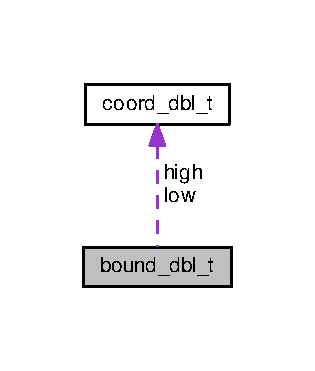
\includegraphics[width=151pt]{d3/daa/structbound__dbl__t__coll__graph}
\end{center}
\end{figure}
\subsection*{Data Fields}
\begin{DoxyCompactItemize}
\item 
\hypertarget{structbound__dbl__t_a77041a08ad4f3d41d695b3f551628561}{}\hyperlink{structcoord__dbl__t}{coord\+\_\+dbl\+\_\+t} {\bfseries low}\label{structbound__dbl__t_a77041a08ad4f3d41d695b3f551628561}

\item 
\hypertarget{structbound__dbl__t_ad4bbe9a305f3911a08647b03ec945195}{}\hyperlink{structcoord__dbl__t}{coord\+\_\+dbl\+\_\+t} {\bfseries high}\label{structbound__dbl__t_ad4bbe9a305f3911a08647b03ec945195}

\end{DoxyCompactItemize}


The documentation for this struct was generated from the following file\+:\begin{DoxyCompactItemize}
\item 
/home/ncasler/apps/\+D\+S\+M\+E/include/bound.\+h\end{DoxyCompactItemize}

\hypertarget{structbound__t}{}\section{bound\+\_\+t Struct Reference}
\label{structbound__t}\index{bound\+\_\+t@{bound\+\_\+t}}


Collaboration diagram for bound\+\_\+t\+:\nopagebreak
\begin{figure}[H]
\begin{center}
\leavevmode
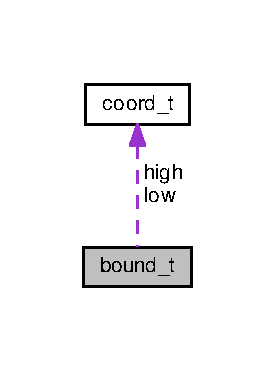
\includegraphics[width=132pt]{d0/d09/structbound__t__coll__graph}
\end{center}
\end{figure}
\subsection*{Data Fields}
\begin{DoxyCompactItemize}
\item 
\hypertarget{structbound__t_a1ed22ec59e044bdee317909ffbe40b59}{}\hyperlink{structcoord__t}{coord\+\_\+t} {\bfseries low}\label{structbound__t_a1ed22ec59e044bdee317909ffbe40b59}

\item 
\hypertarget{structbound__t_afe44f968321b3f4af4db338935a14b1f}{}\hyperlink{structcoord__t}{coord\+\_\+t} {\bfseries high}\label{structbound__t_afe44f968321b3f4af4db338935a14b1f}

\end{DoxyCompactItemize}


The documentation for this struct was generated from the following file\+:\begin{DoxyCompactItemize}
\item 
/home/ncasler/apps/\+D\+S\+M\+E/include/bound.\+h\end{DoxyCompactItemize}

\hypertarget{structcolor__t}{}\section{color\+\_\+t Struct Reference}
\label{structcolor__t}\index{color\+\_\+t@{color\+\_\+t}}
\subsection*{Data Fields}
\begin{DoxyCompactItemize}
\item 
\hypertarget{structcolor__t_aab71f78fa178c16f0140c8341af7b8be}{}short {\bfseries r}\label{structcolor__t_aab71f78fa178c16f0140c8341af7b8be}

\item 
\hypertarget{structcolor__t_ae4a1617d1259807e30d9d28d094f9801}{}short {\bfseries g}\label{structcolor__t_ae4a1617d1259807e30d9d28d094f9801}

\item 
\hypertarget{structcolor__t_a1cf6659d939099119341ce3809a875f3}{}short {\bfseries b}\label{structcolor__t_a1cf6659d939099119341ce3809a875f3}

\end{DoxyCompactItemize}


The documentation for this struct was generated from the following file\+:\begin{DoxyCompactItemize}
\item 
/home/ncasler/apps/\+D\+S\+M\+E/include/point.\+h\end{DoxyCompactItemize}

\hypertarget{structcoord__dbl__t}{}\section{coord\+\_\+dbl\+\_\+t Struct Reference}
\label{structcoord__dbl__t}\index{coord\+\_\+dbl\+\_\+t@{coord\+\_\+dbl\+\_\+t}}
\subsection*{Data Fields}
\begin{DoxyCompactItemize}
\item 
\hypertarget{structcoord__dbl__t_a9d03a2ed64ced526319933f016cfeb4c}{}double {\bfseries x}\label{structcoord__dbl__t_a9d03a2ed64ced526319933f016cfeb4c}

\item 
\hypertarget{structcoord__dbl__t_a32ade1f362b8f0ae140afd4d59dfe7b5}{}double {\bfseries y}\label{structcoord__dbl__t_a32ade1f362b8f0ae140afd4d59dfe7b5}

\item 
\hypertarget{structcoord__dbl__t_af53cc0c637a74448e0b49cbe153474f6}{}double {\bfseries z}\label{structcoord__dbl__t_af53cc0c637a74448e0b49cbe153474f6}

\end{DoxyCompactItemize}


The documentation for this struct was generated from the following file\+:\begin{DoxyCompactItemize}
\item 
/home/ncasler/apps/\+D\+S\+M\+E/include/point.\+h\end{DoxyCompactItemize}

\hypertarget{structcoord__t}{}\section{coord\+\_\+t Struct Reference}
\label{structcoord__t}\index{coord\+\_\+t@{coord\+\_\+t}}
\subsection*{Data Fields}
\begin{DoxyCompactItemize}
\item 
\hypertarget{structcoord__t_a9b55fa0e546159121a030db54021dba6}{}uint32\+\_\+t {\bfseries x}\label{structcoord__t_a9b55fa0e546159121a030db54021dba6}

\item 
\hypertarget{structcoord__t_a1edb2f190d23582bdd512804305d5ecb}{}uint32\+\_\+t {\bfseries y}\label{structcoord__t_a1edb2f190d23582bdd512804305d5ecb}

\item 
\hypertarget{structcoord__t_aa9ad690a5e48f7da6a6a00504916aaaf}{}uint32\+\_\+t {\bfseries z}\label{structcoord__t_aa9ad690a5e48f7da6a6a00504916aaaf}

\end{DoxyCompactItemize}


The documentation for this struct was generated from the following file\+:\begin{DoxyCompactItemize}
\item 
/home/ncasler/apps/\+D\+S\+M\+E/include/point.\+h\end{DoxyCompactItemize}

\hypertarget{structfilter__t}{}\section{filter\+\_\+t Struct Reference}
\label{structfilter__t}\index{filter\+\_\+t@{filter\+\_\+t}}


Collaboration diagram for filter\+\_\+t\+:\nopagebreak
\begin{figure}[H]
\begin{center}
\leavevmode
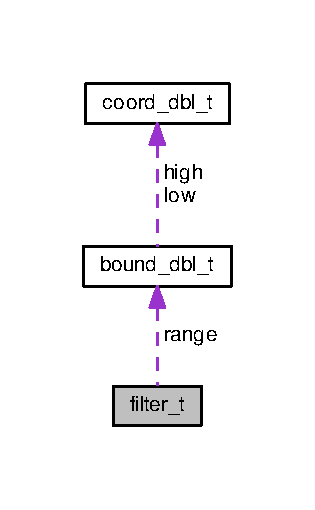
\includegraphics[width=151pt]{dd/d67/structfilter__t__coll__graph}
\end{center}
\end{figure}
\subsection*{Data Fields}
\begin{DoxyCompactItemize}
\item 
\hypertarget{structfilter__t_a16b5a1d44749075caf726bf69a9b5eb5}{}\hyperlink{structbound__dbl__t}{bound\+\_\+dbl\+\_\+t} {\bfseries range}\label{structfilter__t_a16b5a1d44749075caf726bf69a9b5eb5}

\item 
\hypertarget{structfilter__t_a662b0905cd8cad1213d96b1a1d5b73e4}{}int {\bfseries retn}\label{structfilter__t_a662b0905cd8cad1213d96b1a1d5b73e4}

\item 
\hypertarget{structfilter__t_a0e2b54faead36d94f5e00c16388a8d4c}{}int {\bfseries intens}\label{structfilter__t_a0e2b54faead36d94f5e00c16388a8d4c}

\item 
\hypertarget{structfilter__t_acf49d1c252a6444f920ed7c18e5081ea}{}char {\bfseries clas}\label{structfilter__t_acf49d1c252a6444f920ed7c18e5081ea}

\end{DoxyCompactItemize}


The documentation for this struct was generated from the following file\+:\begin{DoxyCompactItemize}
\item 
/home/ncasler/apps/\+D\+S\+M\+E/include/filter.\+h\end{DoxyCompactItemize}

\hypertarget{structHcode}{}\section{Hcode Struct Reference}
\label{structHcode}\index{Hcode@{Hcode}}
\subsection*{Data Fields}
\begin{DoxyCompactItemize}
\item 
\hypertarget{structHcode_a9a4152613f4a4ffc9cee382656c95b21}{}uint32\+\_\+t {\bfseries hcode} \mbox{[}D\+I\+M\mbox{]}\label{structHcode_a9a4152613f4a4ffc9cee382656c95b21}

\end{DoxyCompactItemize}


The documentation for this struct was generated from the following file\+:\begin{DoxyCompactItemize}
\item 
/home/ncasler/apps/\+D\+S\+M\+E/include/hilbert.\+h\end{DoxyCompactItemize}

\hypertarget{structheader__t}{}\section{header\+\_\+t Struct Reference}
\label{structheader__t}\index{header\+\_\+t@{header\+\_\+t}}


Collaboration diagram for header\+\_\+t\+:\nopagebreak
\begin{figure}[H]
\begin{center}
\leavevmode
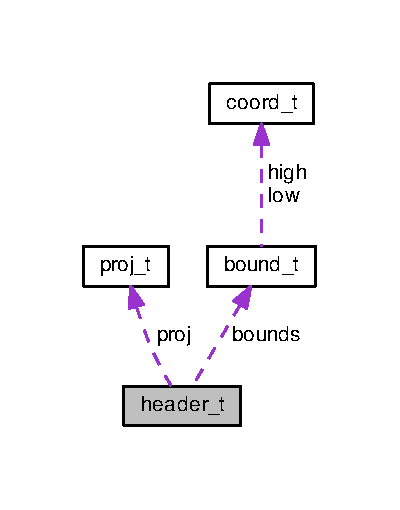
\includegraphics[width=192pt]{d6/d71/structheader__t__coll__graph}
\end{center}
\end{figure}
\subsection*{Data Fields}
\begin{DoxyCompactItemize}
\item 
\hypertarget{structheader__t_a68cac7334ce712d0f88f5c07a13ec090}{}uint32\+\_\+t {\bfseries id}\label{structheader__t_a68cac7334ce712d0f88f5c07a13ec090}

\item 
\hypertarget{structheader__t_ae3f01641558524288a8ee112a35f87eb}{}uint32\+\_\+t {\bfseries pnt\+\_\+count}\label{structheader__t_ae3f01641558524288a8ee112a35f87eb}

\item 
\hypertarget{structheader__t_a2f3027c685ecfa452dd1cd8949a1e7ab}{}\hyperlink{structbound__t}{bound\+\_\+t} {\bfseries bounds}\label{structheader__t_a2f3027c685ecfa452dd1cd8949a1e7ab}

\item 
\hypertarget{structheader__t_a771cbcf21e4a66dfb85e48795562ec82}{}char {\bfseries path} \mbox{[}4096\mbox{]}\label{structheader__t_a771cbcf21e4a66dfb85e48795562ec82}

\item 
\hypertarget{structheader__t_a333dff43bf513368d4cb0ede5e6f9f44}{}\hyperlink{structproj__t}{proj\+\_\+t} {\bfseries proj}\label{structheader__t_a333dff43bf513368d4cb0ede5e6f9f44}

\end{DoxyCompactItemize}


The documentation for this struct was generated from the following file\+:\begin{DoxyCompactItemize}
\item 
/home/ncasler/apps/\+D\+S\+M\+E/include/header.\+h\end{DoxyCompactItemize}

\hypertarget{structJobstat}{}\section{Jobstat Struct Reference}
\label{structJobstat}\index{Jobstat@{Jobstat}}


{\ttfamily \#include $<$util.\+h$>$}

\subsection*{Data Fields}
\begin{DoxyCompactItemize}
\item 
\hypertarget{structJobstat_ada1786a003b0dc56e66dfe9b21ebb00e}{}double {\bfseries Tread}\label{structJobstat_ada1786a003b0dc56e66dfe9b21ebb00e}

\item 
\hypertarget{structJobstat_af277ce2c5fba23904835f4ddcabcb0d1}{}double {\bfseries Tcommdata}\label{structJobstat_af277ce2c5fba23904835f4ddcabcb0d1}

\item 
\hypertarget{structJobstat_ae45f1f3fb3677c761fc75feb90ff8c8a}{}double {\bfseries Tcompute}\label{structJobstat_ae45f1f3fb3677c761fc75feb90ff8c8a}

\item 
\hypertarget{structJobstat_a2197fac600e97d5034757ad75eb0ab39}{}double {\bfseries Tcommresult}\label{structJobstat_a2197fac600e97d5034757ad75eb0ab39}

\item 
\hypertarget{structJobstat_aad5476e2b35b4db54cdec349c25bd1c4}{}double {\bfseries Twrite}\label{structJobstat_aad5476e2b35b4db54cdec349c25bd1c4}

\item 
\hypertarget{structJobstat_aaa924e7bd413313082af0f7921065dcc}{}double {\bfseries Ttotal}\label{structJobstat_aaa924e7bd413313082af0f7921065dcc}

\end{DoxyCompactItemize}


\subsection{Detailed Description}
\hyperlink{util_8h_source}{util.\+h}\+: common utility functions needed for L\+A\+S/\+H\+D\+F read/write Adapted from work by Yan Liu 

The documentation for this struct was generated from the following file\+:\begin{DoxyCompactItemize}
\item 
/home/ncasler/apps/\+D\+S\+M\+E/include/util.\+h\end{DoxyCompactItemize}

\hypertarget{structopdata}{}\section{opdata Struct Reference}
\label{structopdata}\index{opdata@{opdata}}


Collaboration diagram for opdata\+:\nopagebreak
\begin{figure}[H]
\begin{center}
\leavevmode
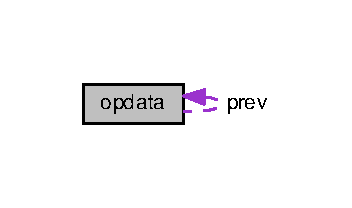
\includegraphics[width=169pt]{da/ddf/structopdata__coll__graph}
\end{center}
\end{figure}
\subsection*{Data Fields}
\begin{DoxyCompactItemize}
\item 
\hypertarget{structopdata_a45e0f6b082939684945a016bbc053507}{}unsigned {\bfseries recurs}\label{structopdata_a45e0f6b082939684945a016bbc053507}

\item 
\hypertarget{structopdata_aca5c8fc54f3ee06a51eb3f9e40ce4b7f}{}struct \hyperlink{structopdata}{opdata} $\ast$ {\bfseries prev}\label{structopdata_aca5c8fc54f3ee06a51eb3f9e40ce4b7f}

\item 
\hypertarget{structopdata_a12e1bf828a0cb70253d508355a825512}{}haddr\+\_\+t {\bfseries addr}\label{structopdata_a12e1bf828a0cb70253d508355a825512}

\end{DoxyCompactItemize}


The documentation for this struct was generated from the following file\+:\begin{DoxyCompactItemize}
\item 
/home/ncasler/apps/\+D\+S\+M\+E/test/check\+Catalog.\+c\end{DoxyCompactItemize}

\hypertarget{structPoint}{}\section{Point Struct Reference}
\label{structPoint}\index{Point@{Point}}


Collaboration diagram for Point\+:\nopagebreak
\begin{figure}[H]
\begin{center}
\leavevmode
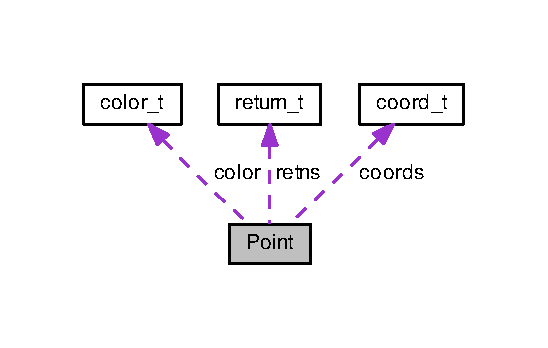
\includegraphics[width=263pt]{dc/d3b/structPoint__coll__graph}
\end{center}
\end{figure}
\subsection*{Data Fields}
\begin{DoxyCompactItemize}
\item 
\hypertarget{structPoint_a55102ae8e345d14df73d7e5e341dda1e}{}uint64\+\_\+t {\bfseries idx}\label{structPoint_a55102ae8e345d14df73d7e5e341dda1e}

\item 
\hypertarget{structPoint_ac8b4f48f5ffbf950e49966f31f76e340}{}\hyperlink{structcoord__t}{coord\+\_\+t} {\bfseries coords}\label{structPoint_ac8b4f48f5ffbf950e49966f31f76e340}

\item 
\hypertarget{structPoint_acae5ade0df0b43fc8728ac4936cc9de1}{}int {\bfseries i}\label{structPoint_acae5ade0df0b43fc8728ac4936cc9de1}

\item 
\hypertarget{structPoint_a019325e9ff1136cd55459356be5835ba}{}\hyperlink{structreturn__t}{return\+\_\+t} {\bfseries retns}\label{structPoint_a019325e9ff1136cd55459356be5835ba}

\item 
\hypertarget{structPoint_ab4a34b7297d6cd29197108e792a4b66f}{}unsigned char {\bfseries clss}\label{structPoint_ab4a34b7297d6cd29197108e792a4b66f}

\item 
\hypertarget{structPoint_a0a95eb2d2f21f0c809d6e27dcd92e335}{}\hyperlink{structcolor__t}{color\+\_\+t} {\bfseries color}\label{structPoint_a0a95eb2d2f21f0c809d6e27dcd92e335}

\end{DoxyCompactItemize}


The documentation for this struct was generated from the following file\+:\begin{DoxyCompactItemize}
\item 
/home/ncasler/apps/\+D\+S\+M\+E/include/point.\+h\end{DoxyCompactItemize}

\hypertarget{structproj__t}{}\section{proj\+\_\+t Struct Reference}
\label{structproj__t}\index{proj\+\_\+t@{proj\+\_\+t}}
\subsection*{Data Fields}
\begin{DoxyCompactItemize}
\item 
\hypertarget{structproj__t_afc1a5828cd65f6831fe6952bbe751fe2}{}char {\bfseries proj4} \mbox{[}4096\mbox{]}\label{structproj__t_afc1a5828cd65f6831fe6952bbe751fe2}

\end{DoxyCompactItemize}


The documentation for this struct was generated from the following file\+:\begin{DoxyCompactItemize}
\item 
/home/ncasler/apps/\+D\+S\+M\+E/include/header.\+h\end{DoxyCompactItemize}

\hypertarget{structreturn__t}{}\section{return\+\_\+t Struct Reference}
\label{structreturn__t}\index{return\+\_\+t@{return\+\_\+t}}
\subsection*{Data Fields}
\begin{DoxyCompactItemize}
\item 
\hypertarget{structreturn__t_a6b36ad9f257a1ea90eeab16eff15796a}{}short {\bfseries r\+Num}\label{structreturn__t_a6b36ad9f257a1ea90eeab16eff15796a}

\item 
\hypertarget{structreturn__t_ae89626627a292c16de890c25378cc5c3}{}short {\bfseries r\+Tot}\label{structreturn__t_ae89626627a292c16de890c25378cc5c3}

\end{DoxyCompactItemize}


The documentation for this struct was generated from the following file\+:\begin{DoxyCompactItemize}
\item 
/home/ncasler/apps/\+D\+S\+M\+E/include/point.\+h\end{DoxyCompactItemize}

\hypertarget{structtask__t}{}\section{task\+\_\+t Struct Reference}
\label{structtask__t}\index{task\+\_\+t@{task\+\_\+t}}
\subsection*{Data Fields}
\begin{DoxyCompactItemize}
\item 
\hypertarget{structtask__t_a4ca575f47056e50da8301683aeeabf9a}{}size\+\_\+t {\bfseries offset}\label{structtask__t_a4ca575f47056e50da8301683aeeabf9a}

\item 
\hypertarget{structtask__t_a2688869cbd5053f91193f75bcbeacc24}{}size\+\_\+t {\bfseries size}\label{structtask__t_a2688869cbd5053f91193f75bcbeacc24}

\item 
\hypertarget{structtask__t_a36787a7e960a588d4a6c4017a0e72a21}{}char {\bfseries fname} \mbox{[}P\+A\+T\+H\+\_\+\+L\+E\+N\mbox{]}\label{structtask__t_a36787a7e960a588d4a6c4017a0e72a21}

\end{DoxyCompactItemize}


The documentation for this struct was generated from the following file\+:\begin{DoxyCompactItemize}
\item 
/home/ncasler/apps/\+D\+S\+M\+E/include/file\+\_\+util.\+h\end{DoxyCompactItemize}

\chapter{File Documentation}
\hypertarget{bound_8c}{}\section{/home/ncasler/apps/\+D\+S\+M\+E/src/bound.c File Reference}
\label{bound_8c}\index{/home/ncasler/apps/\+D\+S\+M\+E/src/bound.\+c@{/home/ncasler/apps/\+D\+S\+M\+E/src/bound.\+c}}


File containing methods for the bound object.  


{\ttfamily \#include $<$mpi.\+h$>$}\\*
{\ttfamily \#include $<$stdio.\+h$>$}\\*
{\ttfamily \#include $<$stdlib.\+h$>$}\\*
{\ttfamily \#include $<$hdf5.\+h$>$}\\*
{\ttfamily \#include \char`\"{}point.\+h\char`\"{}}\\*
{\ttfamily \#include \char`\"{}bound.\+h\char`\"{}}\\*
{\ttfamily \#include \char`\"{}common.\+h\char`\"{}}\\*
{\ttfamily \#include $<$math.\+h$>$}\\*
{\ttfamily \#include $<$inttypes.\+h$>$}\\*
{\ttfamily \#include $<$limits.\+h$>$}\\*
{\ttfamily \#include $<$proj\+\_\+api.\+h$>$}\\*
{\ttfamily \#include $<$liblas/capi/liblas.\+h$>$}\\*
Include dependency graph for bound.\+c\+:
\nopagebreak
\begin{figure}[H]
\begin{center}
\leavevmode
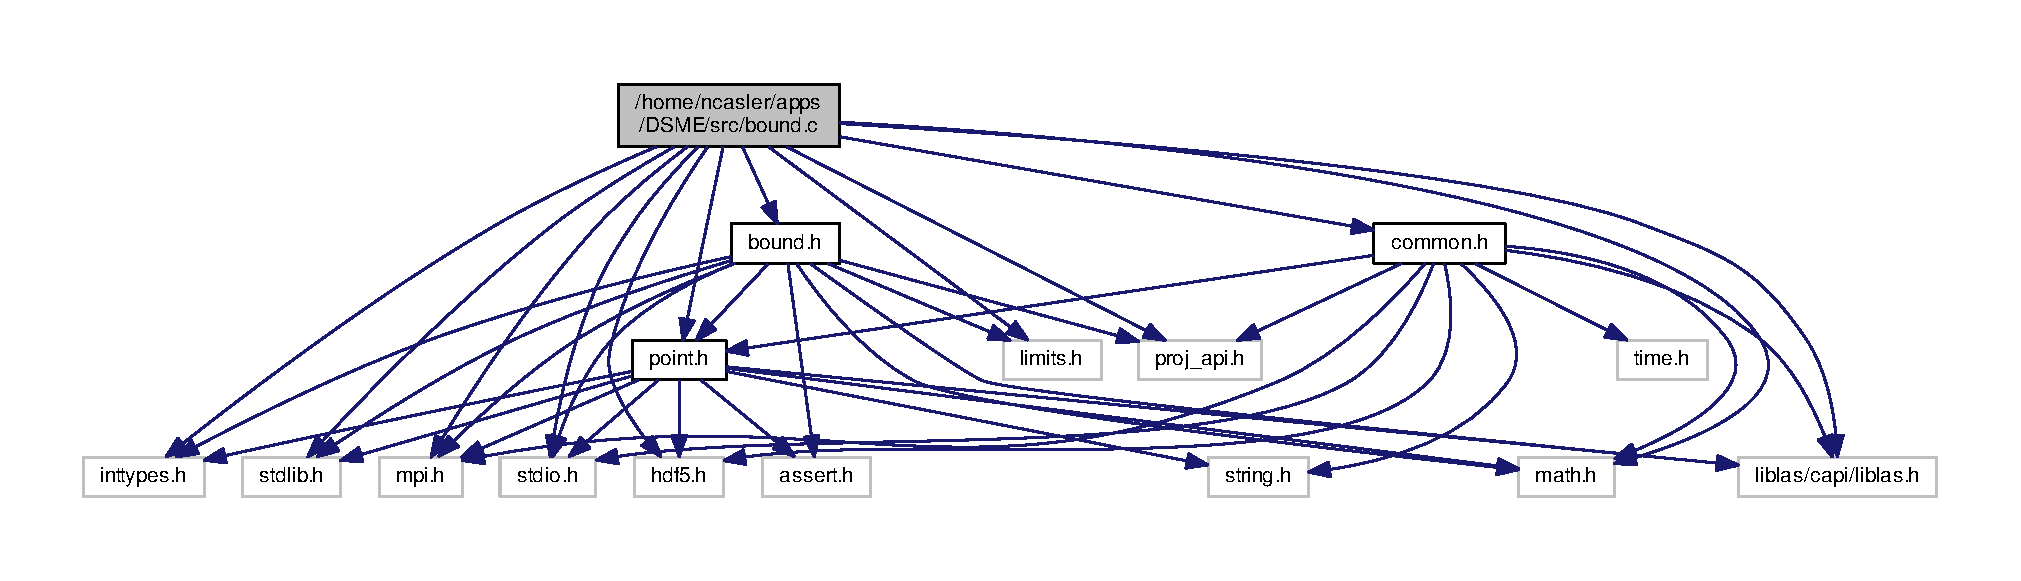
\includegraphics[width=350pt]{d7/d4e/bound_8c__incl}
\end{center}
\end{figure}
\subsection*{Functions}
\begin{DoxyCompactItemize}
\item 
\hypertarget{bound_8c_aa4d70752d75151add9f636f0114a86a4}{}int {\bfseries L\+A\+S\+Bound\+\_\+\+Get} (L\+A\+S\+Header\+H $\ast$header, \hyperlink{structbound__t}{bound\+\_\+t} $\ast$bounds)\label{bound_8c_aa4d70752d75151add9f636f0114a86a4}

\item 
\hypertarget{bound_8c_ac24265ed36340e400af8b9318b784411}{}int {\bfseries Bound\+\_\+intersects} (\hyperlink{structbound__t}{bound\+\_\+t} $\ast$bound\+\_\+1, \hyperlink{structbound__t}{bound\+\_\+t} $\ast$bound\+\_\+2)\label{bound_8c_ac24265ed36340e400af8b9318b784411}

\item 
\hypertarget{bound_8c_a775535bbe269a75ae1406e4759cf95b2}{}hid\+\_\+t {\bfseries Bound\+Type\+\_\+create} (herr\+\_\+t $\ast$status)\label{bound_8c_a775535bbe269a75ae1406e4759cf95b2}

\item 
\hypertarget{bound_8c_a552de3caa3bdee065e2a0acc5b57c21f}{}void {\bfseries Bound\+Type\+\_\+destroy} (hid\+\_\+t boundtype, herr\+\_\+t $\ast$status)\label{bound_8c_a552de3caa3bdee065e2a0acc5b57c21f}

\item 
\hypertarget{bound_8c_afce4730b026d2f2431b6ebe026bae0b4}{}int {\bfseries M\+P\+I\+\_\+\+Bound\+Type\+\_\+create} (M\+P\+I\+\_\+\+Datatype $\ast$mpi\+\_\+boundtype)\label{bound_8c_afce4730b026d2f2431b6ebe026bae0b4}

\item 
\hypertarget{bound_8c_ada897dfcbd0c04171c9f2c29555f0613}{}void {\bfseries Bound\+\_\+dbl\+\_\+\+Set} (\hyperlink{structbound__dbl__t}{bound\+\_\+dbl\+\_\+t} $\ast$bounds, double min\+X, double min\+Y, double min\+Z, double max\+X, double max\+Y, double max\+Z)\label{bound_8c_ada897dfcbd0c04171c9f2c29555f0613}

\item 
int \hyperlink{bound_8c_aeb3c5ace20a27fb04f8669fa2069b638}{Bound\+\_\+dbl\+\_\+\+Project} (\hyperlink{structbound__dbl__t}{bound\+\_\+dbl\+\_\+t} $\ast$bound, L\+A\+S\+S\+R\+S\+H srs)
\end{DoxyCompactItemize}


\subsection{Detailed Description}
File containing methods for the bound object. 

\begin{DoxyAuthor}{Author}
Nathan Casler 
\end{DoxyAuthor}
\begin{DoxyDate}{Date}
6 May 2016 
\end{DoxyDate}


\subsection{Function Documentation}
\hypertarget{bound_8c_aeb3c5ace20a27fb04f8669fa2069b638}{}\index{bound.\+c@{bound.\+c}!Bound\+\_\+dbl\+\_\+\+Project@{Bound\+\_\+dbl\+\_\+\+Project}}
\index{Bound\+\_\+dbl\+\_\+\+Project@{Bound\+\_\+dbl\+\_\+\+Project}!bound.\+c@{bound.\+c}}
\subsubsection[{Bound\+\_\+dbl\+\_\+\+Project}]{\setlength{\rightskip}{0pt plus 5cm}int Bound\+\_\+dbl\+\_\+\+Project (
\begin{DoxyParamCaption}
\item[{{\bf bound\+\_\+dbl\+\_\+t} $\ast$}]{bound, }
\item[{L\+A\+S\+S\+R\+S\+H}]{srs}
\end{DoxyParamCaption}
)}\label{bound_8c_aeb3c5ace20a27fb04f8669fa2069b638}
Bound\+\_\+dbl\+\_\+\+Project\+: Projects a boundary object to a given C\+R\+S 
\begin{DoxyParams}{Parameters}
{\em bound} & \hyperlink{structbound__dbl__t}{bound\+\_\+dbl\+\_\+t} = The bounds to project \\
\hline
{\em srs} & L\+A\+S\+S\+R\+S\+H = The desired projection for the bounds \\
\hline
\end{DoxyParams}
\begin{DoxyReturn}{Returns}
\+: Int 
\end{DoxyReturn}

\hypertarget{common_8c}{}\section{/home/ncasler/apps/\+D\+S\+M\+E/src/common.c File Reference}
\label{common_8c}\index{/home/ncasler/apps/\+D\+S\+M\+E/src/common.\+c@{/home/ncasler/apps/\+D\+S\+M\+E/src/common.\+c}}


File containing common utility functions.  


{\ttfamily \#include \char`\"{}mpi.\+h\char`\"{}}\\*
{\ttfamily \#include \char`\"{}hdf5.\+h\char`\"{}}\\*
{\ttfamily \#include \char`\"{}common.\+h\char`\"{}}\\*
{\ttfamily \#include \char`\"{}point.\+h\char`\"{}}\\*
{\ttfamily \#include \char`\"{}hilbert.\+h\char`\"{}}\\*
{\ttfamily \#include \char`\"{}header.\+h\char`\"{}}\\*
{\ttfamily \#include $<$time.\+h$>$}\\*
{\ttfamily \#include $<$stdio.\+h$>$}\\*
{\ttfamily \#include $<$stdlib.\+h$>$}\\*
{\ttfamily \#include $<$string.\+h$>$}\\*
{\ttfamily \#include $<$math.\+h$>$}\\*
{\ttfamily \#include $<$liblas/capi/liblas.\+h$>$}\\*
{\ttfamily \#include $<$proj\+\_\+api.\+h$>$}\\*
Include dependency graph for common.\+c\+:
\nopagebreak
\begin{figure}[H]
\begin{center}
\leavevmode
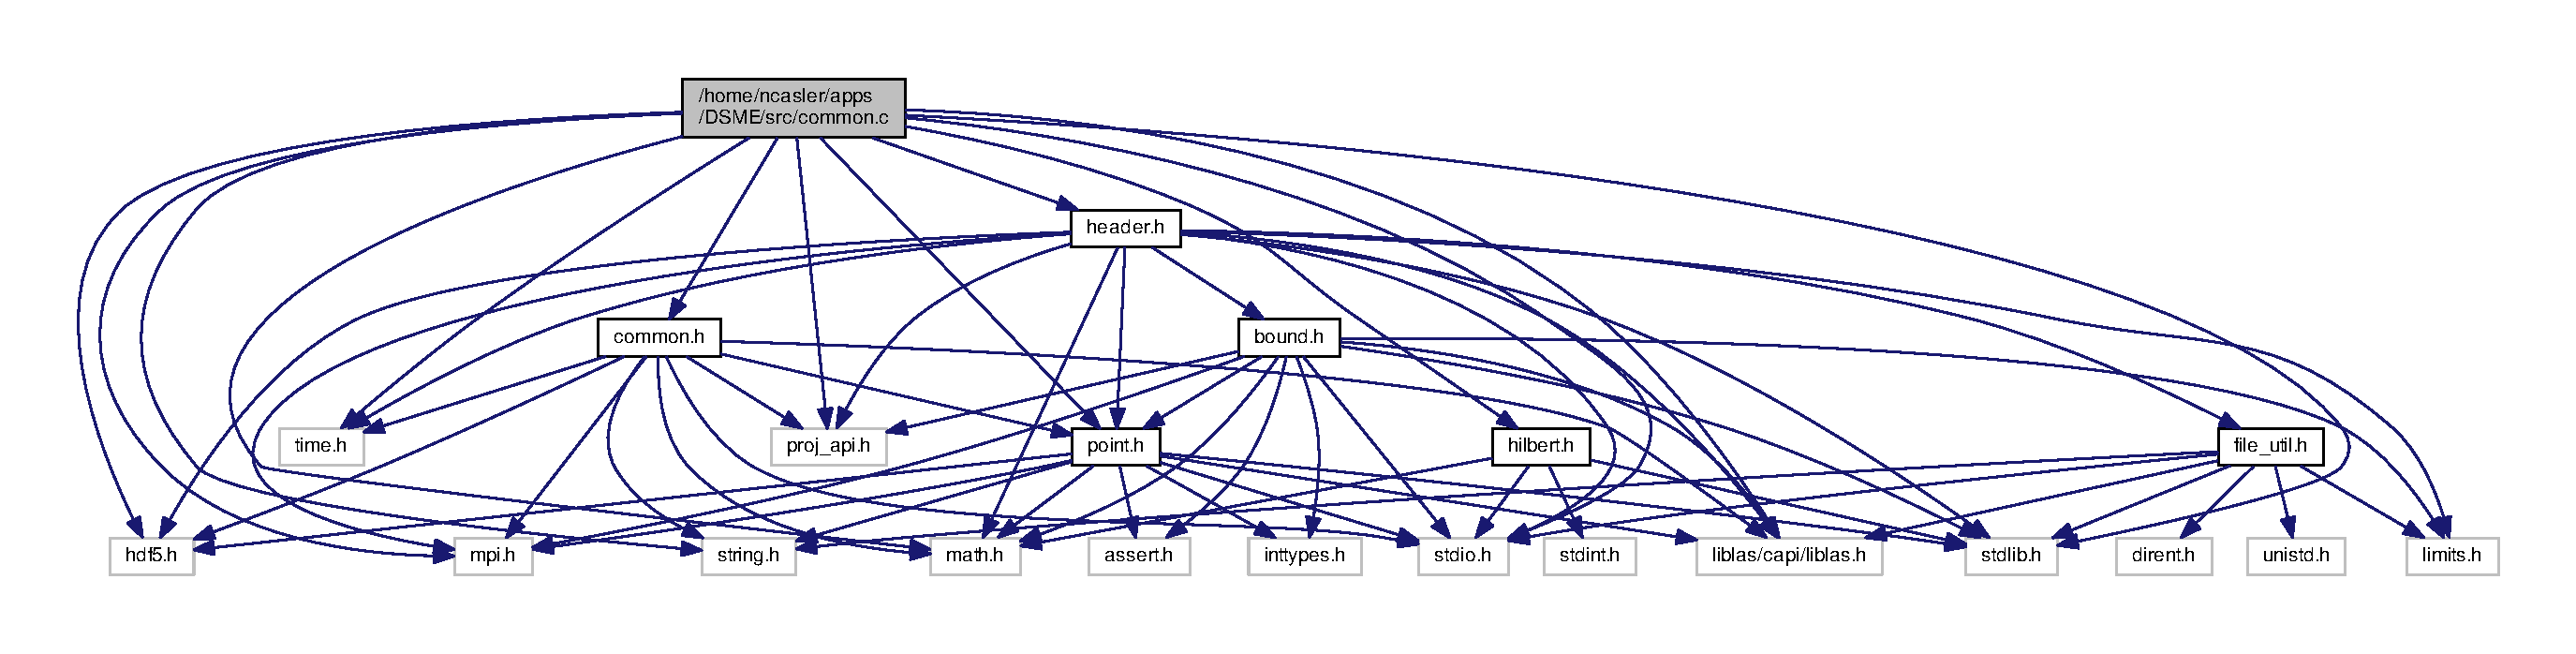
\includegraphics[width=350pt]{d2/dfd/common_8c__incl}
\end{center}
\end{figure}
\subsection*{Functions}
\begin{DoxyCompactItemize}
\item 
int \hyperlink{common_8c_a557143a08234730b391d82c8de6fceaa}{Proj\+\_\+load} (const char $\ast$proj4string, proj\+P\+J $\ast$proj)
\begin{DoxyCompactList}\small\item\em Proj\+\_\+load\+: read a proj\+P\+J object from a Proj.\+4 String. \end{DoxyCompactList}\item 
int \hyperlink{common_8c_a9e784f5c0b1559714371b8f94f72aff5}{L\+A\+S\+Proj\+\_\+get} (L\+A\+S\+Header\+H $\ast$header, proj\+P\+J $\ast$proj)
\begin{DoxyCompactList}\small\item\em L\+A\+S\+Proj\+\_\+get\+: Retrive a proj\+P\+J projection definition from a L\+A\+S file header. \end{DoxyCompactList}\item 
int \hyperlink{common_8c_af3b99206705dde10676fed66ed7c038b}{get\+Point\+Count} (L\+A\+S\+Header\+H header)
\begin{DoxyCompactList}\small\item\em get\+Point\+Count\+: Read the number of points from a L\+A\+S file header \end{DoxyCompactList}\item 
int \hyperlink{common_8c_ab5e30f4f5dc9cfaa334d47bfedef50f8}{project} (proj\+P\+J pj\+\_\+src, proj\+P\+J pj\+\_\+dst, double x, double y, double z)
\begin{DoxyCompactList}\small\item\em project\+: Project a point from one projection to another \end{DoxyCompactList}\item 
int \hyperlink{common_8c_a4dcaae413722189257f43b147220cb00}{create\+Dataset} (char $\ast$file, char $\ast$dataset, hsize\+\_\+t $\ast$dim)
\begin{DoxyCompactList}\small\item\em create\+Dataset\+: Create an H\+D\+F5 dataset witha given name and size \end{DoxyCompactList}\end{DoxyCompactItemize}


\subsection{Detailed Description}
File containing common utility functions. 

\begin{DoxyAuthor}{Author}
Nathan Casler 
\end{DoxyAuthor}
\begin{DoxyDate}{Date}
May 6 2016 
\end{DoxyDate}


\subsection{Function Documentation}
\hypertarget{common_8c_a4dcaae413722189257f43b147220cb00}{}\index{common.\+c@{common.\+c}!create\+Dataset@{create\+Dataset}}
\index{create\+Dataset@{create\+Dataset}!common.\+c@{common.\+c}}
\subsubsection[{create\+Dataset}]{\setlength{\rightskip}{0pt plus 5cm}int create\+Dataset (
\begin{DoxyParamCaption}
\item[{char $\ast$}]{file, }
\item[{char $\ast$}]{dataset, }
\item[{hsize\+\_\+t $\ast$}]{dim}
\end{DoxyParamCaption}
)}\label{common_8c_a4dcaae413722189257f43b147220cb00}


create\+Dataset\+: Create an H\+D\+F5 dataset witha given name and size 


\begin{DoxyParams}{Parameters}
{\em file} & char$\ast$ = Pointer to string containing H\+D\+F5 filename \\
\hline
{\em dataset} & char$\ast$ = Pointer to string containing the desired dataset name \\
\hline
{\em dim} & hsize\+\_\+t$\ast$ = Array containing the lengths of the dataset dimensions \\
\hline
\end{DoxyParams}
Create the return data type

Create the color data type \hypertarget{common_8c_af3b99206705dde10676fed66ed7c038b}{}\index{common.\+c@{common.\+c}!get\+Point\+Count@{get\+Point\+Count}}
\index{get\+Point\+Count@{get\+Point\+Count}!common.\+c@{common.\+c}}
\subsubsection[{get\+Point\+Count}]{\setlength{\rightskip}{0pt plus 5cm}int get\+Point\+Count (
\begin{DoxyParamCaption}
\item[{L\+A\+S\+Header\+H}]{header}
\end{DoxyParamCaption}
)}\label{common_8c_af3b99206705dde10676fed66ed7c038b}


get\+Point\+Count\+: Read the number of points from a L\+A\+S file header 


\begin{DoxyParams}{Parameters}
{\em header} & L\+A\+S\+Header\+H = Header object containing L\+A\+S metadata \\
\hline
\end{DoxyParams}
\begin{DoxyReturn}{Returns}
Int = Number of points in the file 
\end{DoxyReturn}
\hypertarget{common_8c_a9e784f5c0b1559714371b8f94f72aff5}{}\index{common.\+c@{common.\+c}!L\+A\+S\+Proj\+\_\+get@{L\+A\+S\+Proj\+\_\+get}}
\index{L\+A\+S\+Proj\+\_\+get@{L\+A\+S\+Proj\+\_\+get}!common.\+c@{common.\+c}}
\subsubsection[{L\+A\+S\+Proj\+\_\+get}]{\setlength{\rightskip}{0pt plus 5cm}int L\+A\+S\+Proj\+\_\+get (
\begin{DoxyParamCaption}
\item[{L\+A\+S\+Header\+H $\ast$}]{header, }
\item[{proj\+P\+J $\ast$}]{proj}
\end{DoxyParamCaption}
)}\label{common_8c_a9e784f5c0b1559714371b8f94f72aff5}


L\+A\+S\+Proj\+\_\+get\+: Retrive a proj\+P\+J projection definition from a L\+A\+S file header. 


\begin{DoxyParams}{Parameters}
{\em header} & L\+A\+S\+Header\+H$\ast$ = Pointer to L\+A\+S file header \\
\hline
{\em proj} & proj\+P\+J$\ast$ = Pointer to proj\+P\+J object to write the projection definition \\
\hline
\end{DoxyParams}
\begin{DoxyReturn}{Returns}
1 if successful, else 0 
\end{DoxyReturn}
\hypertarget{common_8c_a557143a08234730b391d82c8de6fceaa}{}\index{common.\+c@{common.\+c}!Proj\+\_\+load@{Proj\+\_\+load}}
\index{Proj\+\_\+load@{Proj\+\_\+load}!common.\+c@{common.\+c}}
\subsubsection[{Proj\+\_\+load}]{\setlength{\rightskip}{0pt plus 5cm}int Proj\+\_\+load (
\begin{DoxyParamCaption}
\item[{const char $\ast$}]{proj4string, }
\item[{proj\+P\+J $\ast$}]{proj}
\end{DoxyParamCaption}
)}\label{common_8c_a557143a08234730b391d82c8de6fceaa}


Proj\+\_\+load\+: read a proj\+P\+J object from a Proj.\+4 String. 


\begin{DoxyParams}{Parameters}
{\em proj4string} & const char$\ast$ = Pointer to proj4 string \\
\hline
{\em proj} & proj\+P\+J$\ast$ = Pointer to projection object to write the definition \\
\hline
\end{DoxyParams}
\begin{DoxyReturn}{Returns}
1 if successful, else 0 
\end{DoxyReturn}
\hypertarget{common_8c_ab5e30f4f5dc9cfaa334d47bfedef50f8}{}\index{common.\+c@{common.\+c}!project@{project}}
\index{project@{project}!common.\+c@{common.\+c}}
\subsubsection[{project}]{\setlength{\rightskip}{0pt plus 5cm}int project (
\begin{DoxyParamCaption}
\item[{proj\+P\+J}]{pj\+\_\+src, }
\item[{proj\+P\+J}]{pj\+\_\+dst, }
\item[{double}]{x, }
\item[{double}]{y, }
\item[{double}]{z}
\end{DoxyParamCaption}
)}\label{common_8c_ab5e30f4f5dc9cfaa334d47bfedef50f8}


project\+: Project a point from one projection to another 


\begin{DoxyParams}{Parameters}
{\em pj\+\_\+src} & proj\+P\+J = Source projection definition \\
\hline
{\em pj\+\_\+dst} & proj\+P\+J = Destination projection definition \\
\hline
{\em x} & double = The coordinate on the X-\/axis \\
\hline
{\em y} & double = The coordinate on the Y-\/axis \\
\hline
{\em z} & double = The coordinate on the Z-\/axis \\
\hline
\end{DoxyParams}
\begin{DoxyReturn}{Returns}
0 if projection succeeds, else 1 (T\+O\+D\+O\+: Should probably reverse these return values for consitency) 
\end{DoxyReturn}

\hypertarget{filter_8c}{}\section{/home/ncasler/apps/\+D\+S\+M\+E/src/filter.c File Reference}
\label{filter_8c}\index{/home/ncasler/apps/\+D\+S\+M\+E/src/filter.\+c@{/home/ncasler/apps/\+D\+S\+M\+E/src/filter.\+c}}


File containing point filtration methods.  


{\ttfamily \#include $<$stdlib.\+h$>$}\\*
{\ttfamily \#include $<$stdio.\+h$>$}\\*
{\ttfamily \#include $<$string.\+h$>$}\\*
{\ttfamily \#include $<$mpi.\+h$>$}\\*
{\ttfamily \#include $<$hdf5.\+h$>$}\\*
{\ttfamily \#include $<$math.\+h$>$}\\*
{\ttfamily \#include $<$inttypes.\+h$>$}\\*
{\ttfamily \#include $<$limits.\+h$>$}\\*
{\ttfamily \#include $<$proj\+\_\+api.\+h$>$}\\*
{\ttfamily \#include $<$liblas/capi/liblas.\+h$>$}\\*
{\ttfamily \#include \char`\"{}point.\+h\char`\"{}}\\*
{\ttfamily \#include \char`\"{}bound.\+h\char`\"{}}\\*
{\ttfamily \#include \char`\"{}filter.\+h\char`\"{}}\\*
Include dependency graph for filter.\+c\+:\nopagebreak
\begin{figure}[H]
\begin{center}
\leavevmode
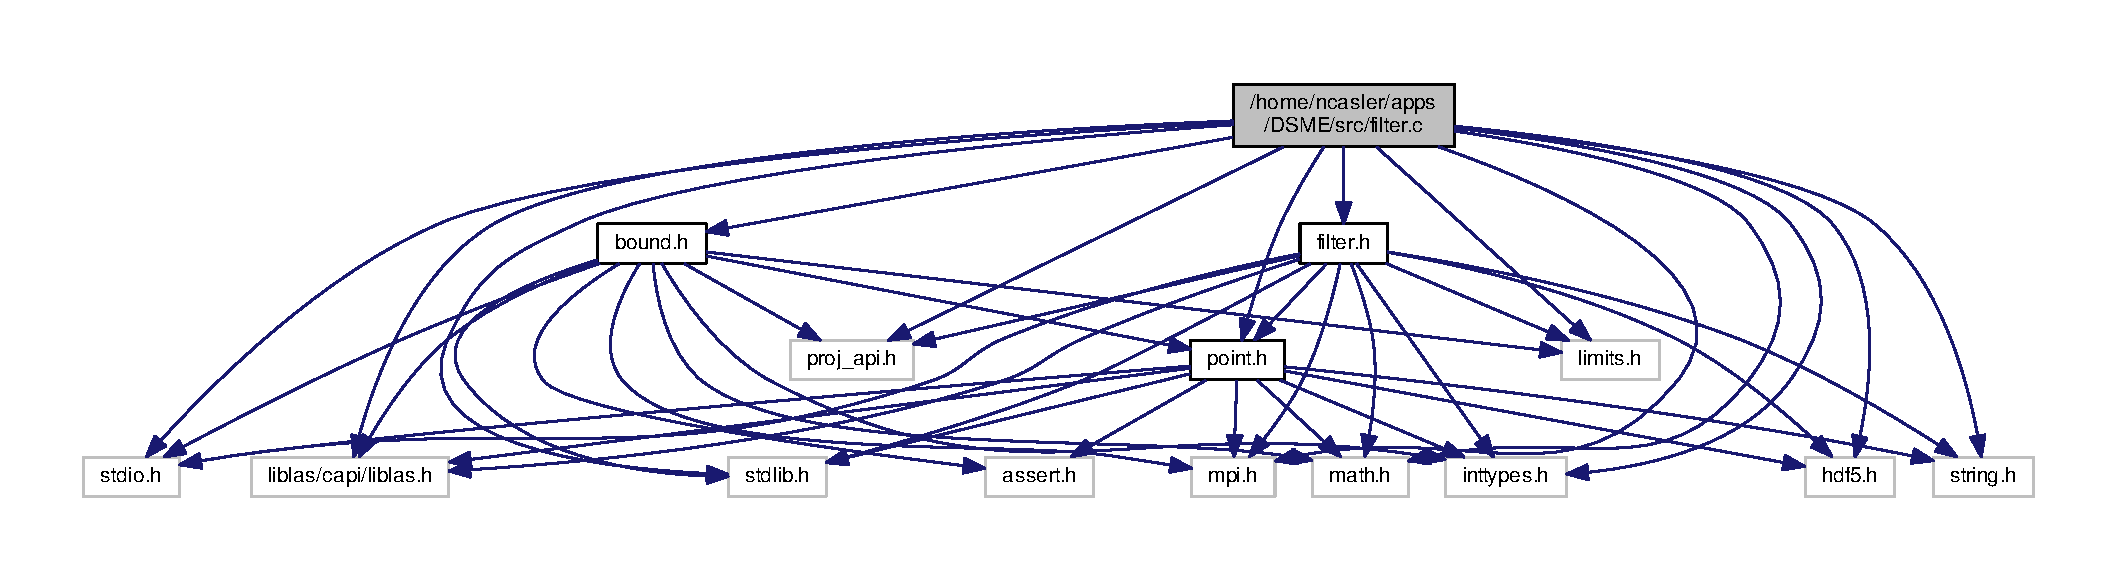
\includegraphics[width=350pt]{d3/d3f/filter_8c__incl}
\end{center}
\end{figure}
\subsection*{Functions}
\begin{DoxyCompactItemize}
\item 
\hyperlink{structfilter__t}{filter\+\_\+t} $\ast$ \hyperlink{filter_8c_a544040ff233d3a5668cb4c3bf944fe07}{Filter\+\_\+\+Create} ()
\begin{DoxyCompactList}\small\item\em Filter\+\_\+\+Create\+: Create a point filter object. \end{DoxyCompactList}\item 
int \hyperlink{filter_8c_a8922cf2ca3820d2fe90fd368e0ee5260}{Filter\+\_\+\+Set} (\hyperlink{structfilter__t}{filter\+\_\+t} $\ast$filter, \hyperlink{structbound__dbl__t}{bound\+\_\+dbl\+\_\+t} $\ast$range, int retn, int intensity, char classification)
\begin{DoxyCompactList}\small\item\em Filter\+\_\+\+Set\+: Setter for filter attributes. \end{DoxyCompactList}\item 
int \hyperlink{filter_8c_a7cba35c3f7dbf4afe72324a99fcda201}{Filter\+\_\+\+Set\+Range} (\hyperlink{structfilter__t}{filter\+\_\+t} $\ast$filter, \hyperlink{structbound__dbl__t}{bound\+\_\+dbl\+\_\+t} $\ast$range)
\begin{DoxyCompactList}\small\item\em Filter\+\_\+\+Set\+Range\+: Set the bounding box for the filter object. \end{DoxyCompactList}\item 
int \hyperlink{filter_8c_ad7f6840636a29296e3c5107472d6b058}{Filter\+\_\+\+Set\+Return} (\hyperlink{structfilter__t}{filter\+\_\+t} $\ast$filter, int retn\+Flag)
\begin{DoxyCompactList}\small\item\em Filter\+\_\+\+Set\+Return\+: Set the return value for the filter object. \end{DoxyCompactList}\item 
void \hyperlink{filter_8c_a115200d003c207903d4749b7497c7e61}{Filter\+\_\+\+Destroy} (\hyperlink{structfilter__t}{filter\+\_\+t} $\ast$filter)
\begin{DoxyCompactList}\small\item\em Filter\+\_\+\+Destroy\+: Frees memory occupied by a filter object. \end{DoxyCompactList}\item 
int \hyperlink{filter_8c_a58d5d30e1986c01faef841b49d47534c}{Filter\+\_\+\+Range\+Check} (\hyperlink{structfilter__t}{filter\+\_\+t} $\ast$filter, L\+A\+S\+Point\+H $\ast$las\+Pnt)
\begin{DoxyCompactList}\small\item\em Filter\+\_\+\+Range\+Check\+: Check if a point falls within bounding filter. \end{DoxyCompactList}\item 
int \hyperlink{filter_8c_a60031cdf106a1a3e338ce4a573a22ee3}{Filter\+\_\+\+Return\+Check} (\hyperlink{structfilter__t}{filter\+\_\+t} $\ast$filter, L\+A\+S\+Point\+H $\ast$las\+Pnt)
\begin{DoxyCompactList}\small\item\em Filter\+\_\+\+Return\+Check\+: Check if a point matches the return filter value. \end{DoxyCompactList}\end{DoxyCompactItemize}


\subsection{Detailed Description}
File containing point filtration methods. 

\begin{DoxyAuthor}{Author}
Nathan Casler 
\end{DoxyAuthor}
\begin{DoxyDate}{Date}
May 6 2016 
\end{DoxyDate}


\subsection{Function Documentation}
\hypertarget{filter_8c_a544040ff233d3a5668cb4c3bf944fe07}{}\index{filter.\+c@{filter.\+c}!Filter\+\_\+\+Create@{Filter\+\_\+\+Create}}
\index{Filter\+\_\+\+Create@{Filter\+\_\+\+Create}!filter.\+c@{filter.\+c}}
\subsubsection[{Filter\+\_\+\+Create}]{\setlength{\rightskip}{0pt plus 5cm}{\bf filter\+\_\+t}$\ast$ Filter\+\_\+\+Create (
\begin{DoxyParamCaption}
{}
\end{DoxyParamCaption}
)}\label{filter_8c_a544040ff233d3a5668cb4c3bf944fe07}


Filter\+\_\+\+Create\+: Create a point filter object. 

\begin{DoxyReturn}{Returns}
filter\+: \hyperlink{structfilter__t}{filter\+\_\+t} = Filter object used to parse a L\+A\+S file 
\end{DoxyReturn}
\hypertarget{filter_8c_a115200d003c207903d4749b7497c7e61}{}\index{filter.\+c@{filter.\+c}!Filter\+\_\+\+Destroy@{Filter\+\_\+\+Destroy}}
\index{Filter\+\_\+\+Destroy@{Filter\+\_\+\+Destroy}!filter.\+c@{filter.\+c}}
\subsubsection[{Filter\+\_\+\+Destroy}]{\setlength{\rightskip}{0pt plus 5cm}void Filter\+\_\+\+Destroy (
\begin{DoxyParamCaption}
\item[{{\bf filter\+\_\+t} $\ast$}]{filter}
\end{DoxyParamCaption}
)}\label{filter_8c_a115200d003c207903d4749b7497c7e61}


Filter\+\_\+\+Destroy\+: Frees memory occupied by a filter object. 


\begin{DoxyParams}{Parameters}
{\em filter} & \hyperlink{structfilter__t}{filter\+\_\+t} = The filter object to free \\
\hline
\end{DoxyParams}
\hypertarget{filter_8c_a58d5d30e1986c01faef841b49d47534c}{}\index{filter.\+c@{filter.\+c}!Filter\+\_\+\+Range\+Check@{Filter\+\_\+\+Range\+Check}}
\index{Filter\+\_\+\+Range\+Check@{Filter\+\_\+\+Range\+Check}!filter.\+c@{filter.\+c}}
\subsubsection[{Filter\+\_\+\+Range\+Check}]{\setlength{\rightskip}{0pt plus 5cm}int Filter\+\_\+\+Range\+Check (
\begin{DoxyParamCaption}
\item[{{\bf filter\+\_\+t} $\ast$}]{filter, }
\item[{L\+A\+S\+Point\+H $\ast$}]{las\+Pnt}
\end{DoxyParamCaption}
)}\label{filter_8c_a58d5d30e1986c01faef841b49d47534c}


Filter\+\_\+\+Range\+Check\+: Check if a point falls within bounding filter. 


\begin{DoxyParams}{Parameters}
{\em filter} & \hyperlink{structfilter__t}{filter\+\_\+t} = The filter holding a range filter \\
\hline
{\em las\+Pnt} & L\+A\+S\+Point\+H = Pointer to a point in a L\+A\+S file \\
\hline
\end{DoxyParams}
\begin{DoxyReturn}{Returns}
1 if point is contained by the filter, else 0 
\end{DoxyReturn}
\begin{DoxyNote}{Note}
\+: There is probably a more efficient/accurate method to do this 
\end{DoxyNote}
\hypertarget{filter_8c_a60031cdf106a1a3e338ce4a573a22ee3}{}\index{filter.\+c@{filter.\+c}!Filter\+\_\+\+Return\+Check@{Filter\+\_\+\+Return\+Check}}
\index{Filter\+\_\+\+Return\+Check@{Filter\+\_\+\+Return\+Check}!filter.\+c@{filter.\+c}}
\subsubsection[{Filter\+\_\+\+Return\+Check}]{\setlength{\rightskip}{0pt plus 5cm}int Filter\+\_\+\+Return\+Check (
\begin{DoxyParamCaption}
\item[{{\bf filter\+\_\+t} $\ast$}]{filter, }
\item[{L\+A\+S\+Point\+H $\ast$}]{las\+Pnt}
\end{DoxyParamCaption}
)}\label{filter_8c_a60031cdf106a1a3e338ce4a573a22ee3}


Filter\+\_\+\+Return\+Check\+: Check if a point matches the return filter value. 


\begin{DoxyParams}{Parameters}
{\em filter} & \hyperlink{structfilter__t}{filter\+\_\+t} = Filter object with a return filter to apply \\
\hline
{\em las\+Pnt} & L\+A\+S\+Point\+H = Pointer to a point in an L\+A\+S file to filter \\
\hline
\end{DoxyParams}
\begin{DoxyReturn}{Returns}
1 if point matches the return filter 
\end{DoxyReturn}
\begin{DoxyNote}{Note}
Currently only matches first or last returns. First if the filter = 1, last if the filter = 2, no matching if filter = 0, else print error 
\end{DoxyNote}
\hypertarget{filter_8c_a8922cf2ca3820d2fe90fd368e0ee5260}{}\index{filter.\+c@{filter.\+c}!Filter\+\_\+\+Set@{Filter\+\_\+\+Set}}
\index{Filter\+\_\+\+Set@{Filter\+\_\+\+Set}!filter.\+c@{filter.\+c}}
\subsubsection[{Filter\+\_\+\+Set}]{\setlength{\rightskip}{0pt plus 5cm}int Filter\+\_\+\+Set (
\begin{DoxyParamCaption}
\item[{{\bf filter\+\_\+t} $\ast$}]{filter, }
\item[{{\bf bound\+\_\+dbl\+\_\+t} $\ast$}]{range, }
\item[{int}]{retn, }
\item[{int}]{intensity, }
\item[{char}]{classification}
\end{DoxyParamCaption}
)}\label{filter_8c_a8922cf2ca3820d2fe90fd368e0ee5260}


Filter\+\_\+\+Set\+: Setter for filter attributes. 

This will set the values for various filter classes 
\begin{DoxyParams}{Parameters}
{\em filter} & \hyperlink{structfilter__t}{filter\+\_\+t} = Filter object to hold settings \\
\hline
{\em range} & \hyperlink{structbound__dbl__t}{bound\+\_\+dbl\+\_\+t} = The bounding box to use when filtering points \\
\hline
{\em retn} & int = The return number to match points against \\
\hline
{\em intensity} & int = The intensity values to match points against \\
\hline
{\em classification} & char = The point classification to read from the points \\
\hline
\end{DoxyParams}
\begin{DoxyReturn}{Returns}
0 
\end{DoxyReturn}
\begin{DoxyNote}{Note}
Should update the return to account for errors(no point or read failure) 

Should update return, intensity and classification to account for ranges of values 
\end{DoxyNote}
\hypertarget{filter_8c_a7cba35c3f7dbf4afe72324a99fcda201}{}\index{filter.\+c@{filter.\+c}!Filter\+\_\+\+Set\+Range@{Filter\+\_\+\+Set\+Range}}
\index{Filter\+\_\+\+Set\+Range@{Filter\+\_\+\+Set\+Range}!filter.\+c@{filter.\+c}}
\subsubsection[{Filter\+\_\+\+Set\+Range}]{\setlength{\rightskip}{0pt plus 5cm}int Filter\+\_\+\+Set\+Range (
\begin{DoxyParamCaption}
\item[{{\bf filter\+\_\+t} $\ast$}]{filter, }
\item[{{\bf bound\+\_\+dbl\+\_\+t} $\ast$}]{range}
\end{DoxyParamCaption}
)}\label{filter_8c_a7cba35c3f7dbf4afe72324a99fcda201}


Filter\+\_\+\+Set\+Range\+: Set the bounding box for the filter object. 


\begin{DoxyParams}{Parameters}
{\em filter} & \hyperlink{structfilter__t}{filter\+\_\+t} = The filter object to update \\
\hline
{\em range} & \hyperlink{structbound__dbl__t}{bound\+\_\+dbl\+\_\+t} = The bounding box to apply to the filter \\
\hline
\end{DoxyParams}
\begin{DoxyReturn}{Returns}
0 
\end{DoxyReturn}
\begin{DoxyNote}{Note}
The range is set in E\+P\+S\+G\+:4326 decimal degrees 
\end{DoxyNote}
\hypertarget{filter_8c_ad7f6840636a29296e3c5107472d6b058}{}\index{filter.\+c@{filter.\+c}!Filter\+\_\+\+Set\+Return@{Filter\+\_\+\+Set\+Return}}
\index{Filter\+\_\+\+Set\+Return@{Filter\+\_\+\+Set\+Return}!filter.\+c@{filter.\+c}}
\subsubsection[{Filter\+\_\+\+Set\+Return}]{\setlength{\rightskip}{0pt plus 5cm}int Filter\+\_\+\+Set\+Return (
\begin{DoxyParamCaption}
\item[{{\bf filter\+\_\+t} $\ast$}]{filter, }
\item[{int}]{retn\+Flag}
\end{DoxyParamCaption}
)}\label{filter_8c_ad7f6840636a29296e3c5107472d6b058}


Filter\+\_\+\+Set\+Return\+: Set the return value for the filter object. 


\begin{DoxyParams}{Parameters}
{\em filter} & \hyperlink{structfilter__t}{filter\+\_\+t} = The filter object to update \\
\hline
{\em retn\+Flag} & int = The return value to set \\
\hline
\end{DoxyParams}
\begin{DoxyReturn}{Returns}
0 
\end{DoxyReturn}

\hypertarget{header_8c}{}\section{/home/ncasler/apps/\+D\+S\+M\+E/src/header.c File Reference}
\label{header_8c}\index{/home/ncasler/apps/\+D\+S\+M\+E/src/header.\+c@{/home/ncasler/apps/\+D\+S\+M\+E/src/header.\+c}}


File containing methods for reading header data.  


{\ttfamily \#include \char`\"{}mpi.\+h\char`\"{}}\\*
{\ttfamily \#include $<$hdf5.\+h$>$}\\*
{\ttfamily \#include \char`\"{}header.\+h\char`\"{}}\\*
{\ttfamily \#include \char`\"{}point.\+h\char`\"{}}\\*
{\ttfamily \#include \char`\"{}file\+\_\+util.\+h\char`\"{}}\\*
{\ttfamily \#include $<$time.\+h$>$}\\*
{\ttfamily \#include $<$stdio.\+h$>$}\\*
{\ttfamily \#include $<$stdlib.\+h$>$}\\*
{\ttfamily \#include $<$string.\+h$>$}\\*
{\ttfamily \#include $<$limits.\+h$>$}\\*
{\ttfamily \#include $<$math.\+h$>$}\\*
{\ttfamily \#include $<$inttypes.\+h$>$}\\*
{\ttfamily \#include $<$liblas/capi/liblas.\+h$>$}\\*
{\ttfamily \#include $<$proj\+\_\+api.\+h$>$}\\*
Include dependency graph for header.\+c\+:
\nopagebreak
\begin{figure}[H]
\begin{center}
\leavevmode
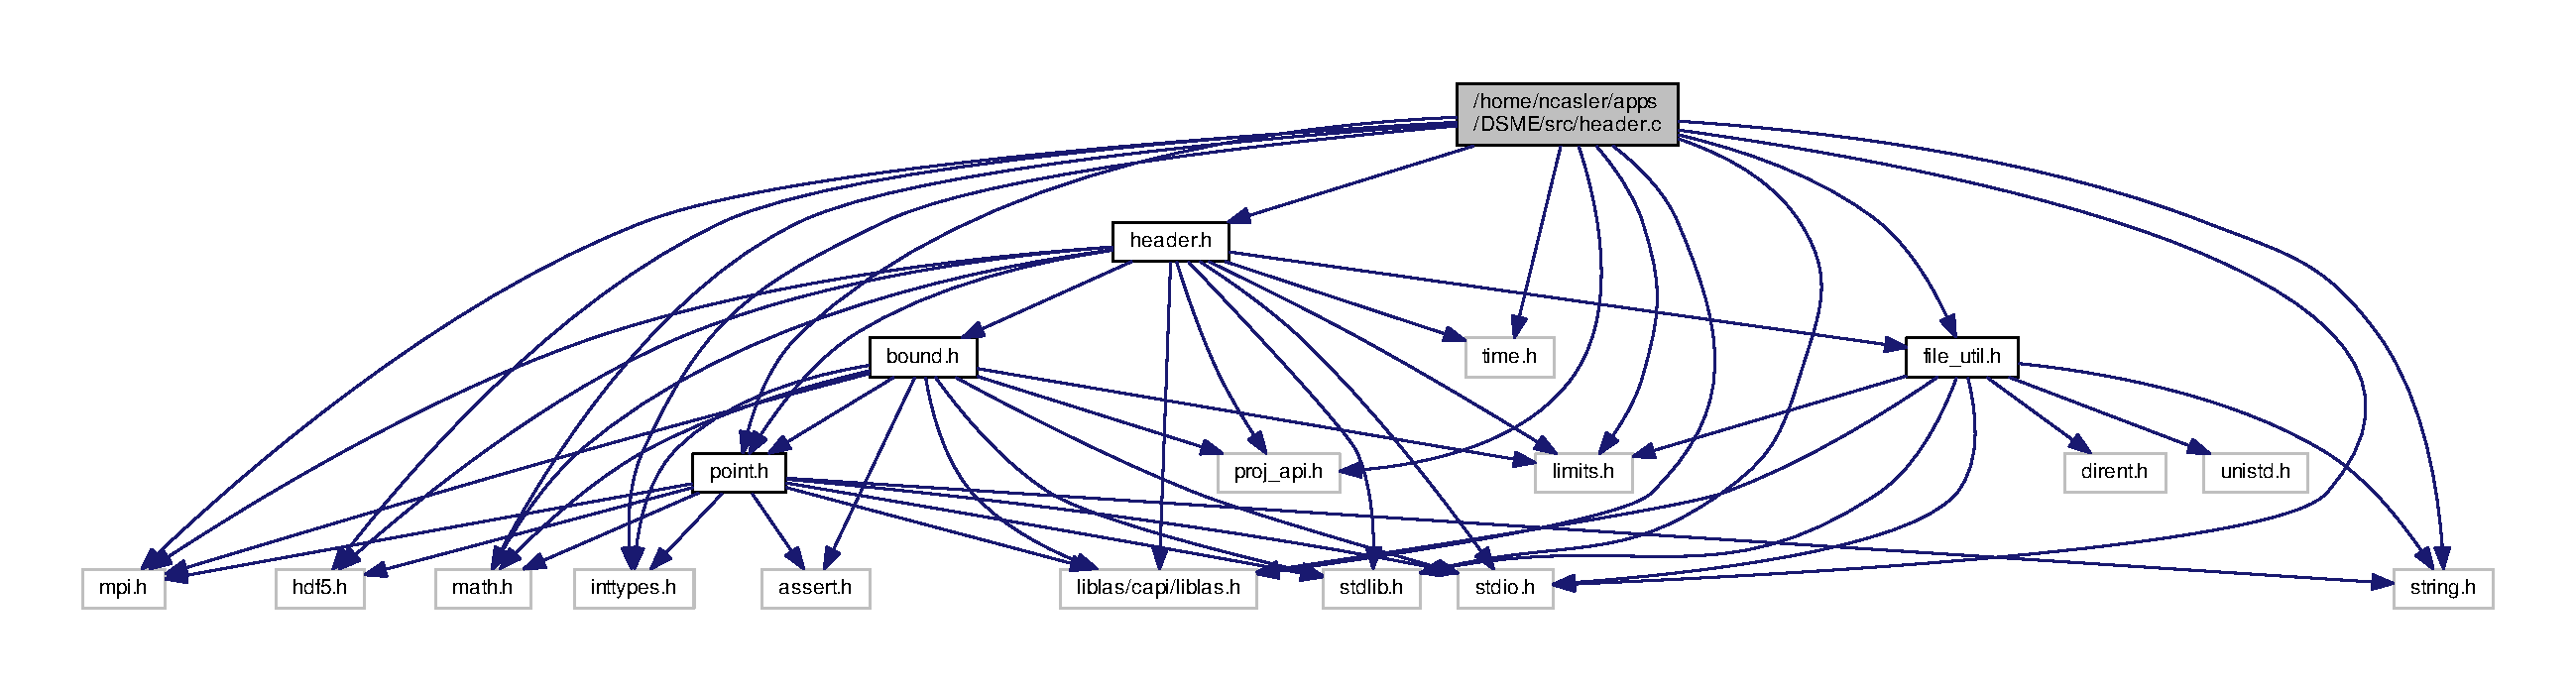
\includegraphics[width=350pt]{df/d03/header_8c__incl}
\end{center}
\end{figure}
\subsection*{Functions}
\begin{DoxyCompactItemize}
\item 
\hypertarget{header_8c_aa037c662039c973fe0694f298bec969f}{}int {\bfseries Proj\+\_\+\+Set} (L\+A\+S\+Header\+H header, \hyperlink{structproj__t}{proj\+\_\+t} $\ast$proj)\label{header_8c_aa037c662039c973fe0694f298bec969f}

\item 
\hypertarget{header_8c_a9237d0239308c6a69d8663b333019079}{}int {\bfseries Header\+\_\+\+Set} (uint32\+\_\+t pnt\+\_\+count, \hyperlink{structbound__t}{bound\+\_\+t} bounds, char fname, \hyperlink{structproj__t}{proj\+\_\+t} proj\+\_\+str)\label{header_8c_a9237d0239308c6a69d8663b333019079}

\item 
\hypertarget{header_8c_a0b98e45139686505241f08f03babc608}{}void {\bfseries Header\+\_\+free} (\hyperlink{structheader__t}{header\+\_\+t} $\ast$headers, int n)\label{header_8c_a0b98e45139686505241f08f03babc608}

\item 
\hypertarget{header_8c_a7ad2b6611184bfd400bdb78e3b39cf96}{}hid\+\_\+t {\bfseries Proj\+Type\+\_\+create} (herr\+\_\+t $\ast$status)\label{header_8c_a7ad2b6611184bfd400bdb78e3b39cf96}

\item 
\hypertarget{header_8c_a7a227a2b71ba6aba2aa1b0a16dd3dffe}{}void {\bfseries Proj\+Type\+\_\+destroy} (hid\+\_\+t projtype, herr\+\_\+t $\ast$status)\label{header_8c_a7a227a2b71ba6aba2aa1b0a16dd3dffe}

\item 
\hypertarget{header_8c_a8feda7283498c28f67fd7e43f7dcd2be}{}hid\+\_\+t {\bfseries Header\+Type\+\_\+create} (herr\+\_\+t $\ast$status)\label{header_8c_a8feda7283498c28f67fd7e43f7dcd2be}

\item 
\hypertarget{header_8c_ac6fe47d3dd42d1f14915387931c733cd}{}void {\bfseries Header\+Type\+\_\+destroy} (hid\+\_\+t headertype, herr\+\_\+t $\ast$status)\label{header_8c_ac6fe47d3dd42d1f14915387931c733cd}

\item 
\hypertarget{header_8c_a37241ac20ee32a58a36056ef51af8f13}{}int {\bfseries M\+P\+I\+\_\+\+Proj\+Type\+\_\+create} (M\+P\+I\+\_\+\+Datatype $\ast$mpi\+\_\+projtype)\label{header_8c_a37241ac20ee32a58a36056ef51af8f13}

\item 
int \hyperlink{header_8c_a0ab5a4a85b76b52f0aecbd8675acd0e1}{M\+P\+I\+\_\+\+Header\+Type\+\_\+create} (M\+P\+I\+\_\+\+Datatype $\ast$mpi\+\_\+headertype)
\item 
int \hyperlink{header_8c_ac1403287a52ddd06dc9b68efc5a855c7}{create\+Header\+Dataset} (char $\ast$file, char $\ast$dataset, hsize\+\_\+t $\ast$dims)
\item 
int \hyperlink{header_8c_a92ffdae1875d58f64540714ae6d2064e}{Header\+\_\+read} (char $\ast$path, \hyperlink{structheader__t}{header\+\_\+t} $\ast$header, uint32\+\_\+t id)
\item 
\hypertarget{header_8c_afb6e7bd488fbae6399ed7ed07f26a1d6}{}int {\bfseries read\+Header\+Block} (char paths\mbox{[}$\,$\mbox{]}, int offset, int block, \hyperlink{structheader__t}{header\+\_\+t} $\ast$headers)\label{header_8c_afb6e7bd488fbae6399ed7ed07f26a1d6}

\item 
\hypertarget{header_8c_aed2201f138398716f4be800c8a150cab}{}int {\bfseries write\+Header\+Block\+\_\+ser} (hid\+\_\+t file\+\_\+id, char $\ast$dataset, hsize\+\_\+t $\ast$offset, hsize\+\_\+t $\ast$block, \hyperlink{structheader__t}{header\+\_\+t} $\ast$headers)\label{header_8c_aed2201f138398716f4be800c8a150cab}

\item 
\hypertarget{header_8c_a2141b90acc4f4bf4c4e2d53a81c43d01}{}int {\bfseries write\+Header\+Block} (hid\+\_\+t file\+\_\+id, char $\ast$dataset, hsize\+\_\+t $\ast$offset, hsize\+\_\+t $\ast$block, \hyperlink{structheader__t}{header\+\_\+t} $\ast$headers, M\+P\+I\+\_\+\+Comm comm, M\+P\+I\+\_\+\+Info info)\label{header_8c_a2141b90acc4f4bf4c4e2d53a81c43d01}

\end{DoxyCompactItemize}


\subsection{Detailed Description}
File containing methods for reading header data. 

\begin{DoxyAuthor}{Author}
Nathan Casler 
\end{DoxyAuthor}
\begin{DoxyDate}{Date}
May 6 2016 
\end{DoxyDate}


\subsection{Function Documentation}
\hypertarget{header_8c_ac1403287a52ddd06dc9b68efc5a855c7}{}\index{header.\+c@{header.\+c}!create\+Header\+Dataset@{create\+Header\+Dataset}}
\index{create\+Header\+Dataset@{create\+Header\+Dataset}!header.\+c@{header.\+c}}
\subsubsection[{create\+Header\+Dataset}]{\setlength{\rightskip}{0pt plus 5cm}int create\+Header\+Dataset (
\begin{DoxyParamCaption}
\item[{char $\ast$}]{file, }
\item[{char $\ast$}]{dataset, }
\item[{hsize\+\_\+t $\ast$}]{dims}
\end{DoxyParamCaption}
)}\label{header_8c_ac1403287a52ddd06dc9b68efc5a855c7}
Set the maximum size, should be an unlimited length 1-\/d array

Set the chunking dimensions, should be tested for perfomance

For T\+E\+S\+T\+I\+N\+G P\+U\+R\+P\+O\+S\+E\+S O\+N\+L\+Y \hypertarget{header_8c_a92ffdae1875d58f64540714ae6d2064e}{}\index{header.\+c@{header.\+c}!Header\+\_\+read@{Header\+\_\+read}}
\index{Header\+\_\+read@{Header\+\_\+read}!header.\+c@{header.\+c}}
\subsubsection[{Header\+\_\+read}]{\setlength{\rightskip}{0pt plus 5cm}int Header\+\_\+read (
\begin{DoxyParamCaption}
\item[{char $\ast$}]{path, }
\item[{{\bf header\+\_\+t} $\ast$}]{header, }
\item[{uint32\+\_\+t}]{id}
\end{DoxyParamCaption}
)}\label{header_8c_a92ffdae1875d58f64540714ae6d2064e}
This function will read the necessary header data from a given L\+A\+S file \hypertarget{header_8c_a0ab5a4a85b76b52f0aecbd8675acd0e1}{}\index{header.\+c@{header.\+c}!M\+P\+I\+\_\+\+Header\+Type\+\_\+create@{M\+P\+I\+\_\+\+Header\+Type\+\_\+create}}
\index{M\+P\+I\+\_\+\+Header\+Type\+\_\+create@{M\+P\+I\+\_\+\+Header\+Type\+\_\+create}!header.\+c@{header.\+c}}
\subsubsection[{M\+P\+I\+\_\+\+Header\+Type\+\_\+create}]{\setlength{\rightskip}{0pt plus 5cm}int M\+P\+I\+\_\+\+Header\+Type\+\_\+create (
\begin{DoxyParamCaption}
\item[{M\+P\+I\+\_\+\+Datatype $\ast$}]{mpi\+\_\+headertype}
\end{DoxyParamCaption}
)}\label{header_8c_a0ab5a4a85b76b52f0aecbd8675acd0e1}
T\+O\+D\+O\+: Fix this struct creation, application quits here 
\hypertarget{hilbert_8c}{}\section{/home/ncasler/apps/\+D\+S\+M\+E/src/hilbert.c File Reference}
\label{hilbert_8c}\index{/home/ncasler/apps/\+D\+S\+M\+E/src/hilbert.\+c@{/home/ncasler/apps/\+D\+S\+M\+E/src/hilbert.\+c}}


File containing point filtration methods.  


{\ttfamily \#include $<$limits.\+h$>$}\\*
{\ttfamily \#include $<$stdlib.\+h$>$}\\*
{\ttfamily \#include $<$stdio.\+h$>$}\\*
{\ttfamily \#include $<$stdint.\+h$>$}\\*
{\ttfamily \#include $<$inttypes.\+h$>$}\\*
{\ttfamily \#include $<$math.\+h$>$}\\*
{\ttfamily \#include $<$hilbert.\+h$>$}\\*
Include dependency graph for hilbert.\+c\+:
\nopagebreak
\begin{figure}[H]
\begin{center}
\leavevmode
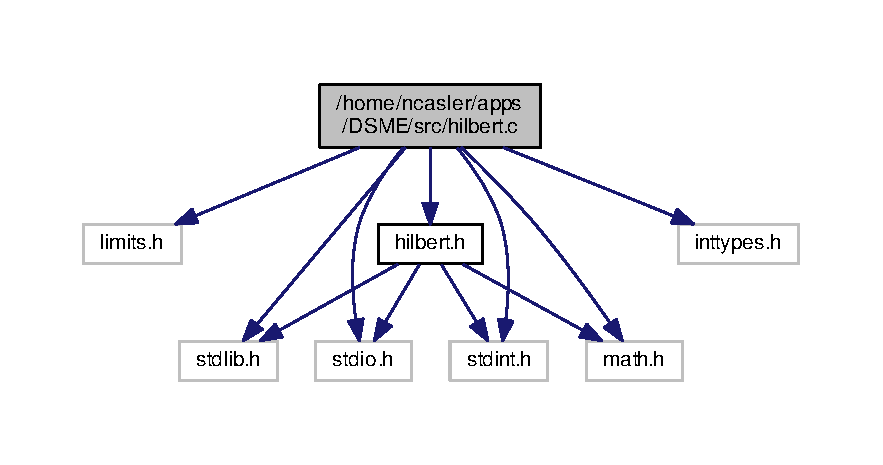
\includegraphics[width=350pt]{d8/d59/hilbert_8c__incl}
\end{center}
\end{figure}
\subsection*{Macros}
\begin{DoxyCompactItemize}
\item 
\hypertarget{hilbert_8c_a89d7ab05b964fcb47cc1adacdedb16d7}{}\#define {\bfseries H\+I\+L\+B\+E\+R\+T\+\_\+\+C}\label{hilbert_8c_a89d7ab05b964fcb47cc1adacdedb16d7}

\item 
\hypertarget{hilbert_8c_ac25189db92959bff3c6c2adf4c34b50a}{}\#define {\bfseries D\+I\+M}~2\label{hilbert_8c_ac25189db92959bff3c6c2adf4c34b50a}

\end{DoxyCompactItemize}
\subsection*{Functions}
\begin{DoxyCompactItemize}
\item 
\hypertarget{hilbert_8c_aed2497e6ce866dec2ff4d41a2727fdc5}{}uint32\+\_\+t {\bfseries calc\+\_\+\+P} (int i, \hyperlink{structHcode}{Hcode} H)\label{hilbert_8c_aed2497e6ce866dec2ff4d41a2727fdc5}

\item 
\hypertarget{hilbert_8c_a5bff2ba44cd4447e908be15e77da9344}{}uint32\+\_\+t {\bfseries calc\+\_\+\+P2} (uint32\+\_\+t S)\label{hilbert_8c_a5bff2ba44cd4447e908be15e77da9344}

\item 
\hypertarget{hilbert_8c_a68c18d125efaa872bdc210bea75acd39}{}uint32\+\_\+t {\bfseries calc\+\_\+\+J} (uint32\+\_\+t P)\label{hilbert_8c_a68c18d125efaa872bdc210bea75acd39}

\item 
\hypertarget{hilbert_8c_ac55f94c438fc03d434456acbf917f704}{}uint32\+\_\+t {\bfseries calc\+\_\+\+T} (uint32\+\_\+t P)\label{hilbert_8c_ac55f94c438fc03d434456acbf917f704}

\item 
\hypertarget{hilbert_8c_a52c238f8b861f83bcf6755fbf4f0c713}{}uint32\+\_\+t {\bfseries calc\+\_\+t\+S\+\_\+t\+T} (uint32\+\_\+t x\+J, uint32\+\_\+t val)\label{hilbert_8c_a52c238f8b861f83bcf6755fbf4f0c713}

\item 
\hypertarget{hilbert_8c_a45daeada8537bc237f0ebf6400a947f6}{}\hyperlink{structHcode}{Hpoint} {\bfseries H\+\_\+decode} (\hyperlink{structHcode}{Hcode} H)\label{hilbert_8c_a45daeada8537bc237f0ebf6400a947f6}

\item 
\hypertarget{hilbert_8c_a3ee110a1b25fe07bbdd5366d990d6f2a}{}\hyperlink{structHcode}{Hcode} {\bfseries H\+\_\+encode} (\hyperlink{structHcode}{Hpoint} pt)\label{hilbert_8c_a3ee110a1b25fe07bbdd5366d990d6f2a}

\item 
\hypertarget{hilbert_8c_a553dc49f84a0874f09d55f9e84fb31d2}{}void {\bfseries print\+Bits} (size\+\_\+t const size, void const $\ast$const ptr)\label{hilbert_8c_a553dc49f84a0874f09d55f9e84fb31d2}

\item 
\hypertarget{hilbert_8c_ad064a5ddb6f9344e748b4541b3e86f27}{}int {\bfseries combine\+Indices} (uint64\+\_\+t $\ast$out\+Idx, uint32\+\_\+t high, uint32\+\_\+t low)\label{hilbert_8c_ad064a5ddb6f9344e748b4541b3e86f27}

\item 
int \hyperlink{hilbert_8c_af28b8fb4b7618175ba6ba11b4e15a506}{less\+\_\+than} (uint64\+\_\+t a, uint64\+\_\+t b)
\item 
\hypertarget{hilbert_8c_a8bbe5cca8f3ca305e402546026a4ad39}{}unsigned {\bfseries create\+Mask} (unsigned start, unsigned stop)\label{hilbert_8c_a8bbe5cca8f3ca305e402546026a4ad39}

\end{DoxyCompactItemize}
\subsection*{Variables}
\begin{DoxyCompactItemize}
\item 
\hypertarget{hilbert_8c_a5ab0e23ad716bd39c51f54dda5a020a2}{}const uint32\+\_\+t {\bfseries g\+\_\+mask} \mbox{[}$\,$\mbox{]} = \{2, 1\}\label{hilbert_8c_a5ab0e23ad716bd39c51f54dda5a020a2}

\end{DoxyCompactItemize}


\subsection{Detailed Description}
File containing point filtration methods. 

\begin{DoxyAuthor}{Author}
Nathan Casler 
\end{DoxyAuthor}
\begin{DoxyDate}{Date}
May 6 2016 Code copied from J.\+K. Lawder, Calculation of Mappings between One and n-\/dimensional Values Using the Hilbert Space-\/filling Curve, Research Report J\+L1/00, School of Computer Science and Information Systems, Birkbeck College, University of London, 2000
\end{DoxyDate}
This code assumes the following

The macro O\+R\+D\+E\+R corresponds to the order of curve and is 32, thus coordinates are 32bit values.

A uint32\+\_\+t should be a 32bit unsigned integer.

The macro D\+I\+M corresponds tot he number of dimensions in a space.

The derived-\/key of a Hpoint is stored in an \hyperlink{structHcode}{Hcode} which is an array of uint32\+\_\+t. The bottom bit of a derived-\/key is held in the bottom bit of the hcode\mbox{[}0\mbox{]} element of an \hyperlink{structHcode}{Hcode} and the top bit of a derived-\/key is held in the top bit of the hcode\mbox{[}D\+I\+M-\/1\mbox{]} element of and \hyperlink{structHcode}{Hcode}.

g\+\_\+mask is a global array of masks which helps simplify some calculations -\/ it has D\+I\+M elements. In each element, only one bit is zeo valued -\/ the top bit in element no. 0 and the bottom bit in element no. (D\+I\+M -\/ 1). eg. \#if D\+I\+M == 5 const uint32\+\_\+t g\+\_\+mask\mbox{[}\mbox{]} = \{16, 8, 4, 2, 1\}; \#endif \#if D\+I\+M == 6 const uint32\+\_\+t g\+\_\+mask\mbox{[}\mbox{]} = \{32, 16, 8, 4, 2, 1\}; \#endif etc... 

\subsection{Function Documentation}
\hypertarget{hilbert_8c_af28b8fb4b7618175ba6ba11b4e15a506}{}\index{hilbert.\+c@{hilbert.\+c}!less\+\_\+than@{less\+\_\+than}}
\index{less\+\_\+than@{less\+\_\+than}!hilbert.\+c@{hilbert.\+c}}
\subsubsection[{less\+\_\+than}]{\setlength{\rightskip}{0pt plus 5cm}int less\+\_\+than (
\begin{DoxyParamCaption}
\item[{uint64\+\_\+t}]{a, }
\item[{uint64\+\_\+t}]{b}
\end{DoxyParamCaption}
)}\label{hilbert_8c_af28b8fb4b7618175ba6ba11b4e15a506}
T\+O\+D\+O\+: M\+A\+K\+E T\+H\+E S\+C\+A\+L\+E C\+O\+N\+V\+E\+R\+S\+I\+O\+N W\+O\+R\+K F\+O\+R F\+L\+O\+A\+T A\+R\+R\+A\+Y void scale\+Coords(double {\itshape coords, Hpoint} pt) \{ uint32\+\_\+t lat\+Off = 90.\+0f, lon\+Off = 180.\+0f, alt\+Off = 12300.\+0f; double offsets\mbox{[}3\mbox{]} = \{180.\+0, 90.\+0, 12300.\+0\}; printf(\char`\"{}\+U\+I\+N\+T\+M\+A\+X\+: \%lf\textbackslash{}n\char`\"{}, U\+I\+N\+T\+\_\+\+M\+A\+X); printf(\char`\"{}\+Input coordinates\+: \%lf, \%lf, \%lf\textbackslash{}n\char`\"{}, coords\mbox{[}0\mbox{]}, coords\mbox{[}1\mbox{]}, coords\mbox{[}2\mbox{]}); int i; uint32\+\_\+t scales\mbox{[}3\mbox{]};

for (i = 0; i $<$ 3; i++) \{ \begin{DoxyVerb}printf("Scaling coord %d\n", i);
double range = 2.0 * offsets[i];
double max = (double)UINT_MAX;
double scale = max / range;
double outCoord = scale * coords[i];
printf("%lf / %lf = %lf\n", max, range, scale);
printf("Out: %lf\n", outCoord);
scales[i] = floor(max / range);
\end{DoxyVerb}
 printf(\char`\"{}\+Scale \%d is\+: \%u, offset\+: \%f\textbackslash{}n\char`\"{}, i, scales\mbox{[}i\mbox{]}, offsets\mbox{[}i\mbox{]});

\begin{DoxyVerb}    printf("Offset coord[%d] is %f\n", i, (coords[i] + offsets[i]));
    pt->hcode[i] = (uint32_t)((coords[i] + offsets[i]) * scales[i]);
    printf("Coord %d has value %lu\n", i, pt->hcode[i]);
}    
\end{DoxyVerb}


\} 
%--- End generated contents ---

% Index
\backmatter
\newpage
\phantomsection
\clearemptydoublepage
\addcontentsline{toc}{chapter}{Index}
\printindex

\end{document}
